\documentclass[11pt,a4paper]{article}
\usepackage[T1]{fontenc}
\usepackage[utf8]{inputenc}
\usepackage[polish]{babel}
\usepackage{amsmath}
\usepackage{amsfonts}
\usepackage{graphicx}
\usepackage[margin=0.8in]{geometry} % for custom margins
\author{Kamil Kuczaj}
\title{Sprawozdanie z Laboratorium 7 - Pomiar czasu wyszukiwania losowego elementu w drzewie binarnym.}
\date{\today}
\begin{document}

\maketitle

\section{Wstęp}
\hspace{4ex}Zadaniem na laboratorium był pomiar czasu wyszukiwania losowego elementu w drzewie czerwono-czarnym (\textit{ang. Red Black Tree}. Drzewo to zostało opracowane przez Rudolfa Bayera w 1972 roku. Wg teorii algorytm wyszukiwania elementu w tej strukturze powinien mieć złożoność obliczeniową równą O($log(n)$).\\\\W naszym przypadku mieliśmy załadować kolejno $10^1$, $10^3$, $10^5$, $10^6$, $10^9$ oraz sprawdzić czas wyszukiwania znanego elementu. Niestety komputer przy próbie alokacji miliarda elementów zapełniał cała pamięć fizyczną RAM komputera i dalsze ładowanie elementów następowało bardzo powoli. Odczyt z tych obszarów pamięci (pliku stronicowego \textit{swap}) zajmował również więcej czasu, co wpłynęło by negatywnie na wyniki pomiarów. Dlatego zdecydowałem się robić pomiary $10^8$ elementów zamiast $10^9$. Ich alokacja kończyła się na zapełnieniu ok. $6,5 GB$ pamięci RAM. W każdej z 50 prób wyszukiwane było to samo słowo, które zostało wylosowane podczas budowania drzewa korzystając z biblioteki \textit{<cstdlib>}.\\\\Obok tzw. \textit{Red Black Tree} możemy znaleźć w literaturze inne konstrukcje (w nawiasach rok opracowania):
\begin{enumerate}
\item AVL tree (1962)
\item B-tree (1972)
\item Scapegoat tree (1989)
\item WAVL tree (2015)
\item Splay tree (1985)
\end{enumerate}
\bigskip
Jednak drzewo czerwono-czarne jest tak świetnym pomysłem, że twórcy języka C++ postanowili je zaimplementować jako element biblioteki STL w postaci \textit{std::set<>}. Pomiary zostały wykonane właśnie na tej konstrukcji ze względu na najpewniejszą dokładność pomiarów.
\section{Specyfikacja komputera}

\begin{center}
	\begin{tabular}{| r | c |}
	\hline
	Wersja kompilatora \textit{g++} & 4.8.4 \\ \hline
	System & Ubuntu 14.04.4 \\ \hline
	Procesor	 & Intel Core i5 2510M 2.3 GHz \\ \hline
	Pamięć RAM & 8 GB DDR3 1600 MHz \\ \hline
	Dysk twardy & HDD (5400 obr./min) \\ \hline
	Rozmiar zmiennej \textit{int} & 4 bajty \\ \hline
	\end{tabular}
\end{center}
\newpage
\section{Pomiary oraz ich interpretacja}

\begin{table}[htbp]
\caption{}
\begin{center}
\begin{tabular}{|c|c|c|c|c|c|}
\hline
\textbf{} & \multicolumn{ 5}{c|}{\textbf{Czasy dla znajdywania elementu w milisekundach}} \\ \hline
\textbf{Ilość elementów} & \textbf{10} & \textbf{1000} & \textbf{100000} & \textbf{1000000} & \textbf{100000000} \\ \hline
\textbf{Pomiar 1 [ms]} & 33 & 28 & 32 & 29 & 26 \\ \hline
\textbf{Pomiar 2 [ms]} & 30 & 30 & 31 & 29 & 28 \\ \hline
\textbf{Pomiar 3 [ms]} & 40 & 24 & 26 & 15 & 10 \\ \hline
\textbf{Pomiar 4 [ms]} & 18 & 28 & 10 & 14 & 7 \\ \hline
\textbf{Pomiar 5 [ms]} & 25 & 22 & 7 & 11 & 7 \\ \hline
\textbf{Pomiar 6 [ms]} & 17 & 24 & 7 & 13 & 7 \\ \hline
\textbf{Pomiar 7 [ms]} & 17 & 23 & 10 & 14 & 7 \\ \hline
\textbf{Pomiar 8 [ms]} & 16 & 22 & 7 & 12 & 7 \\ \hline
\textbf{Pomiar 9 [ms]} & 17 & 23 & 6 & 18 & 7 \\ \hline
\textbf{Pomiar 10 [ms]} & 17 & 24 & 6 & 12 & 7 \\ \hline
\textbf{Pomiar 11 [ms]} & 17 & 23 & 7 & 12 & 8 \\ \hline
\textbf{Pomiar 12 [ms]} & 19 & 23 & 7 & 13 & 7 \\ \hline
\textbf{Pomiar 13 [ms]} & 17 & 23 & 6 & 12 & 7 \\ \hline
\textbf{Pomiar 14 [ms]} & 18 & 33 & 6 & 14 & 7 \\ \hline
\textbf{Pomiar 15 [ms]} & 16 & 23 & 7 & 11 & 7 \\ \hline
\textbf{Pomiar 16 [ms]} & 16 & 23 & 7 & 12 & 7 \\ \hline
\textbf{Pomiar 17 [ms]} & 16 & 23 & 7 & 12 & 7 \\ \hline
\textbf{Pomiar 18 [ms]} & 16 & 28 & 7 & 10 & 6 \\ \hline
\textbf{Pomiar 19 [ms]} & 19 & 24 & 7 & 8 & 7 \\ \hline
\textbf{Pomiar 20 [ms]} & 16 & 20 & 7 & 7 & 7 \\ \hline
\textbf{Pomiar 21 [ms]} & 16 & 18 & 8 & 7 & 7 \\ \hline
\textbf{Pomiar 22 [ms]} & 17 & 19 & 11 & 7 & 7 \\ \hline
\textbf{Pomiar 23 [ms]} & 20 & 20 & 7 & 7 & 7 \\ \hline
\textbf{Pomiar 24 [ms]} & 16 & 18 & 7 & 7 & 7 \\ \hline
\textbf{Pomiar 25 [ms]} & 16 & 21 & 7 & 7 & 7 \\ \hline
\textbf{Pomiar 26 [ms]} & 16 & 18 & 7 & 7 & 7 \\ \hline
\textbf{Pomiar 27 [ms]} & 17 & 18 & 7 & 7 & 8 \\ \hline
\textbf{Pomiar 28 [ms]} & 16 & 18 & 7 & 7 & 7 \\ \hline
\textbf{Pomiar 29 [ms]} & 17 & 19 & 10 & 7 & 7 \\ \hline
\textbf{Pomiar 30 [ms]} & 16 & 18 & 6 & 7 & 7 \\ \hline
\textbf{Pomiar 31 [ms]} & 17 & 18 & 7 & 7 & 7 \\ \hline
\textbf{Pomiar 32 [ms]} & 17 & 19 & 7 & 7 & 8 \\ \hline
\textbf{Pomiar 33 [ms]} & 19 & 17 & 7 & 7 & 7 \\ \hline
\textbf{Pomiar 34 [ms]} & 17 & 18 & 7 & 7 & 9 \\ \hline
\end{tabular}
\end{center}
\label{Wyniki1}
\end{table}

\newpage

\begin{table}[htbp]
\caption{}
\begin{center}
\begin{tabular}{|c|c|c|c|c|c|}
\hline
\textbf{} & \multicolumn{ 5}{c|}{\textbf{Czasy dla znajdywania elementu w milisekundach}} \\ \hline
\textbf{Ilość elementów} & \textbf{10} & \textbf{1000} & \textbf{100000} & \textbf{1000000} & \textbf{100000000} \\ \hline
\textbf{Pomiar 35 [ms]} & 16 & 18 & 7 & 7 & 7 \\ \hline
\textbf{Pomiar 36 [ms]} & 20 & 18 & 8 & 6 & 8 \\ \hline
\textbf{Pomiar 37 [ms]} & 16 & 17 & 7 & 6 & 8 \\ \hline
\textbf{Pomiar 38 [ms]} & 17 & 17 & 6 & 7 & 7 \\ \hline
\textbf{Pomiar 39 [ms]} & 34 & 18 & 6 & 7 & 8 \\ \hline
\textbf{Pomiar 40 [ms]} & 27 & 18 & 6 & 7 & 7 \\ \hline
\textbf{Pomiar 41 [ms]} & 22 & 18 & 7 & 7 & 7 \\ \hline
\textbf{Pomiar 42 [ms]} & 22 & 18 & 7 & 7 & 8 \\ \hline
\textbf{Pomiar 43 [ms]} & 21 & 18 & 7 & 7 & 7 \\ \hline
\textbf{Pomiar 44 [ms]} & 23 & 18 & 7 & 7 & 8 \\ \hline
\textbf{Pomiar 45 [ms]} & 21 & 18 & 7 & 7 & 7 \\ \hline
\textbf{Pomiar 46 [ms]} & 22 & 18 & 7 & 6 & 7 \\ \hline
\textbf{Pomiar 47 [ms]} & 23 & 18 & 6 & 7 & 7 \\ \hline
\textbf{Pomiar 48 [ms]} & 25 & 18 & 7 & 7 & 8 \\ \hline
\textbf{Pomiar 49 [ms]} & 23 & 18 & 7 & 7 & 7 \\ \hline
\textbf{Pomiar 50 [ms]} & 22 & 19 & 8 & 7 & 7 \\ \hline
\end{tabular}
\end{center}
\label{Wyniki2}
\end{table}

\begin{table}[htbp]
\caption{}
\begin{center}
\begin{tabular}{|r|c|}
\hline
\multicolumn{1}{|l|}{\textbf{Ilość elementów}} & \multicolumn{1}{c|}{\textbf{Średni czas na podstawie 50 pomiarów w milisekundach [ms]}} \\ \hline
\textbf{10} & 19,82 \\ \hline
\textbf{1000} & 20,74 \\ \hline
\textbf{100000} & 8,5 \\ \hline
\textbf{1000000} & 9,7 \\ \hline
\textbf{100000000} & 8,06 \\ \hline
\end{tabular}
\end{center}
\label{Wyniki3}
\end{table}


\begin{figure}[htbp]
\begin{center}
	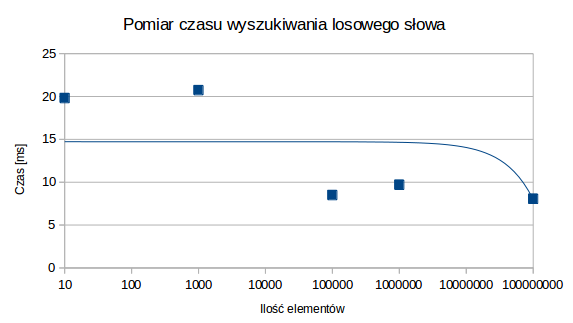
\includegraphics[scale=0.7]{../wyniki/wykres.png}
\end{center}
\caption{Uśrednione wyniki pomiarów wraz z regresją liniową. Oś odciętych w skali logarytmicznej.}
\end{figure}

Wyraźnie widać, że algorytm wyszukiwania odbiega od teorii. Po głębszej analizie biblioteki STL okazało się, że \textit{std::set<>} nie zawsze musi być implementowane jako drzewo czerwono-czarne. W moim przypadku jest to najprawdopodobniej odmiana tablicy asocjacyjnej, gdyż wyniki wskazują na to, iż algorytm wyszukiwania ma złożoność liczbową O($1$). Być może miało tu miejsce również tzw. przewidywanie gałęzi (\textit{ang. Branch Prediction}. Jest to zjawisko, które jest obecne w nowszych systemach jądrach systemu. System mając posortowane dane, lepiej i szybciej radzi sobie z ich przetwarzaniem.

\newpage

\section{Wnioski}
\hspace{4ex}Wyniki nie są zgodne z teorią. Drzewo czerwono-czarne jest bardzo popularną implementacją drzewa binarnego, które nie wymaga rebalansowania. Jest jednak niezmiernie trudne w implementacji, czego przekonano się podczas próby zaprogramowania tej struktury. Nie zdecydowano się na pomiar zwykłego drzewa bez rebalansowania, gdyż najprawdopodobniej otrzymano by złożoność obliczeniową O($n$) z wiadomych względów.
 
\end{document}